% Owner: Khalid  |  Task: T4, T15  |  Drafted by ORCA agents, finalised by the owner.
% Rules: prose only; every claim cited with \citet/\citep to a literature/sources.yaml record id;
% compare methods (G6); strengths/weaknesses/applicability (G8). See tasks/todo.md.
\section{Introduction}
\label{sec:intro}

Knowledge distillation (KD) trains a small student network to match the outputs of a larger teacher, so that
the student keeps much of the teacher's accuracy with lower inference cost \citep{hinton2015kd}. The
original recipe adds a temperature-softened Kullback--Leibler term to the cross-entropy loss. Logit methods split the KD loss into parts and reweight them
\citep{zhao2022dkd}, standardise or rescale logits \citep{sun2024lskd} or learn the temperature
\citep{li2023ctkd}. Feature and relation methods align intermediate representations or the structure between
samples \citep{tian2020crd,chen2022simkd,zhang2025vrm}. Other work changes the training scheme, asks when the
teacher should be trusted at all, or changes how the task gradient and the distillation gradient are combined
\citep{zhao2023dot,hayder2026dtokd}.

\paragraph{Motivation and gap.} Most of this work reports results on the same few teacher--student pairs: CIFAR-100 with the
teacher--student pairs of CRD \citep{tian2020crd} and ImageNet-1K with ResNet34$\to$ResNet18. Yet numbers
from different papers are rarely put side by side with their caveats, and recent gains are often within a
point of each other. Table~\ref{tab:surveys} compares this survey with existing ones: the broad KD surveys \citep{gou2021kdsurvey,wang2022kdreview} predate most methods covered here, \citet{mansourian2025kdsurvey} covers newer work. None of them builds its method set
from a stated search, and none treats the combination of task and distillation objectives as a
multi-objective optimisation problem in its own section. The general MOO survey by \citet{chen2026gradmoo} reviews gradient-combination rules but does not discuss distillation.

\paragraph{Scope and inclusion criteria.} We survey state-of-the-art KD for image classification published
from 2022 to 2026. A paper is included when it meets three criteria fixed before the search. \begin{description}
\item[ I1 ] It proposes a KD method for image classification in which a student uses teacher-provided or internally generated targets. Logit or loss, feature or relation, training scheme, teacher reliability, and objective combination are overlapping analytic dimensions, not exclusive classes. Analysis-only papers support the discussion but are not ranked.
\item[ I2 ] It appeared between January 2022 and the search cutoff, 8 November 2026 at CVPR, ICCV, ECCV, NeurIPS, ICML, ICLR, AAAI, TMLR, TPAMI or IJCV, or is an arXiv preprint first posted from 2025 without such a venue.
\item[ I3 ] It reports top-1 accuracy on CIFAR-100 with a standard CRD teacher--student pair, or on ImageNet-1K with ResNet34$\to$ResNet18 or ResNet50$\to$MobileNetV1.
\end{description}
Exclusion codes are:
\begin{description}
\setlength{\itemsep}{0pt}
\item[E1] Not KD, or KD used only as a tool for another task.
\item[E2] Not image classification.
\item[E3] Venue or date outside I2.
\item[E4] No standard-protocol result.
\item[E5] Survey or position paper.
\item[E6] Dataset distillation or compression without a teacher.
\item[E7] Withdrawn or duplicate version.
\end{description}
Distillation for language models, vision--language models,
detection and other tasks is outside the scope; Section~\ref{sec:future} gives pointers.

\paragraph{Search.} Three searches covered the computer-vision venues, the machine-learning venues and
TMLR, and AAAI, the two journals and arXiv, with snowballing from recent comparison tables. They identified 2,193 records (656, 985 and 552), and 310 were read in full. A
second pass with broader title terms (``teach'', ``student'', ``mimic'', ``logit'' and others) screened 445
further records, re-checked 29 cited works that no search had included, and added two methods. Fifteen
papers that were first inaccessible were later retrieved by hand and added six more. The final set has
112 included records; two papers could not be assessed because no full text was found. An independent spot-check found no errors in 20 accessible sampled inclusions and 20 accessible sampled exclusions. Two additional sampled inclusions and ten sampled exclusions could not be read. The supplementary material gives
each search's sources, queries, date and counts (Table~S1), the per-record screening logs, and the complete list
of the 112 included records with each one's reported results and source table (Table~S2); the main text cites
only the methods it discusses (Fig.~\ref{fig:search-flow}).

\begin{figure}[t]
\centering
\resizebox{\linewidth}{!}{% Search and screening flow. Counts and inclusion arithmetic are in Supplement S1.
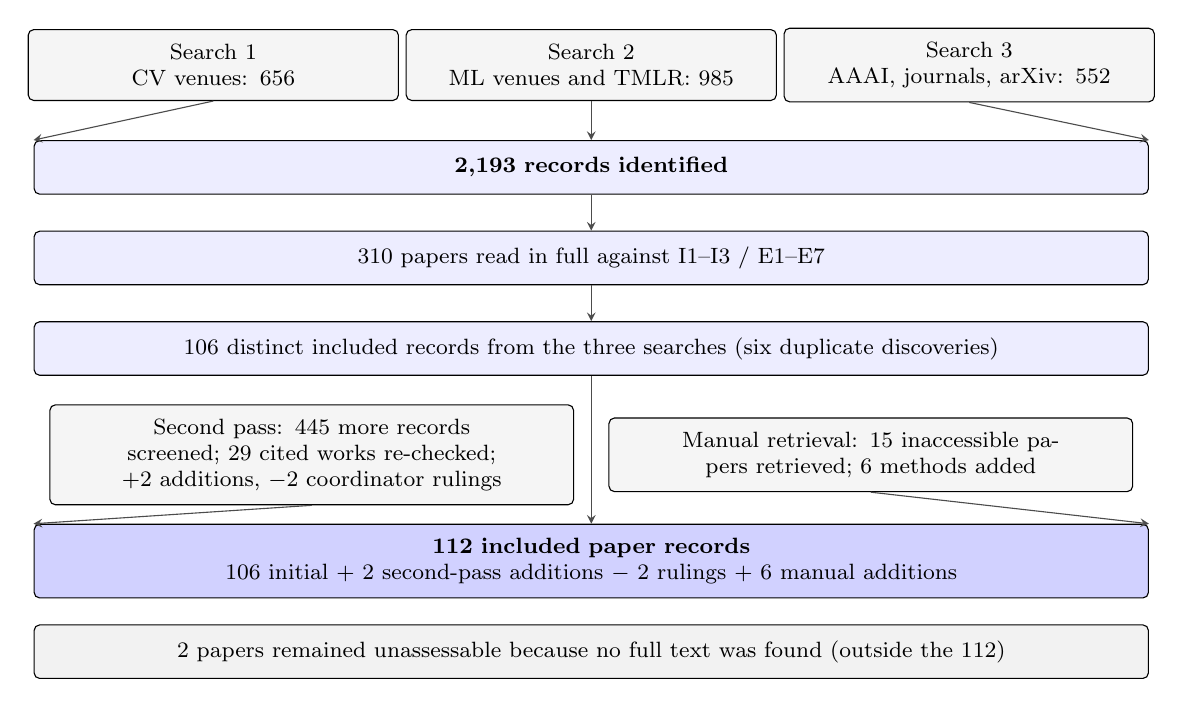
\begin{tikzpicture}[x=1cm,y=-1cm,font=\footnotesize,>=stealth,
  source/.style={draw,rounded corners=2pt,fill=gray!8,align=center,inner sep=5pt,text width=4.35cm,minimum height=0.9cm},
  box/.style={draw,rounded corners=2pt,fill=blue!7,align=center,inner sep=5pt,text width=13.8cm,minimum height=0.68cm},
  side/.style={draw,rounded corners=2pt,fill=gray!8,align=center,inner sep=5pt,text width=6.3cm,minimum height=0.9cm},
  ar/.style={->,>=stealth,black!70,thin}]
  \node[source] (s1) at (-4.8,0) {Search 1\\CV venues: 656};
  \node[source] (s2) at (0,0) {Search 2\\ML venues and TMLR: 985};
  \node[source] (s3) at (4.8,0) {Search 3\\AAAI, journals, arXiv: 552};
  \node[box] (identified) at (0,1.3) {\textbf{2,193 records identified}};
  \node[box] (screened) at (0,2.45) {310 papers read in full against I1--I3 / E1--E7};
  \node[box] (distinct) at (0,3.6) {106 distinct included records from the three searches (six duplicate discoveries)};
  \node[side] (second) at (-3.55,4.95) {Second pass: 445 more records screened; 29 cited works re-checked; +2 additions, $-$2 coordinator rulings};
  \node[side] (manual) at (3.55,4.95) {Manual retrieval: 15 inaccessible papers retrieved; 6 methods added};
  \node[box,fill=blue!18] (included) at (0,6.3) {\textbf{112 included paper records}\\106 initial + 2 second-pass additions $-$ 2 rulings + 6 manual additions};
  \node[box,fill=gray!10] (unavailable) at (0,7.45) {2 papers remained unassessable because no full text was found (outside the 112)};
  \draw[ar] (s1.south) -- (identified.north west);
  \draw[ar] (s2.south) -- (identified.north);
  \draw[ar] (s3.south) -- (identified.north east);
  \draw[ar] (identified) -- (screened);
  \draw[ar] (screened) -- (distinct);
  \draw[ar] (distinct) -- (included);
  \draw[ar] (second.south) -- (included.north west);
  \draw[ar] (manual.south) -- (included.north east);
\end{tikzpicture}
}
\caption{Search and screening flow from three source groups through full-text screening and inclusion. The second pass and manual retrieval update the included set; the two unassessable papers remain outside it. I1--I3 and E1--E7 are the inclusion and exclusion criteria.}
\label{fig:search-flow}
\end{figure}

\paragraph{Taxonomy.} Figure~\ref{fig:taxonomy} shows how the methods are organised. These dimensions overlap: methods may be described by the knowledge transferred (logits in Section~\ref{sec:logit}, or features and relations in Section~\ref{sec:feature}); the training scheme (offline, online, self-distillation, multi-teacher or data-free); teacher reliability; and rules that combine task and distillation gradients (Sections~\ref{sec:moo} and~\ref{sec:kd_moo}).

\paragraph{Contributions.} The survey makes four contributions. First, it gives a set of included paper records for 2022--2026
built from a documented search with fixed criteria, so a reader can check why a method is in or out.
Second, it describes each family with its strengths, weaknesses and applicability. Third, it reviews multi-objective optimisation for distillation and compares KD methods that use it with general gradient-combination rules. PCD \citep{varam2026pcd} is included as a candidate general rule; it has no reported distillation evaluation, and gradient conflict in standard distillation remains largely untested (\S\ref{sec:kd_moo_critical}). Fourth, it
collects the reported CIFAR-100 and ImageNet numbers of the included methods in one place and flags the rows
whose setting differs from the standard protocol.

Section~\ref{sec:benchmarks} compiles the reported results, Section~\ref{sec:future} discusses open
challenges, and the supplementary material lists all included methods.

% --- Table I / Fig. 1 (T4) --- (per-cell evidence: docs/survey/table1-evidence.md)
% Every cell is justified by a section number of the compared survey in docs/survey/table1-evidence.md.
% The "This survey" row states the coverage planned in tasks/plan.md (Secs. sec:logit..sec:benchmarks).
\newcommand{\tY}{$\checkmark$}
\newcommand{\tP}{$\circ$}
\newcommand{\tN}{$\times$}
\begin{table}[htbp]
\centering
\caption{Comparison with existing surveys. \tY: covered in a dedicated section; \tP: covered
partially or only in a narrower setting; \tN: not covered. ``MOO in KD'': the distillation and task objectives
treated with multi-objective optimisation (Pareto, gradient balancing or conflict handling); loss
weighting alone counts as \tP. ``2024--26'': discusses knowledge-distillation methods published in
2024--2026.}
\label{tab:surveys}
\small
\setlength{\tabcolsep}{3.5pt}
\begin{tabular}{llccccccccc}
\toprule
Survey & Venue & Year & Logit & \shortstack{Feat./\\relation} & Schemes & \shortstack{Teacher\\reliab.} &
  \shortstack{MOO\\in KD} & \shortstack{Bench./\\results} & \shortstack{LLM/\\VLM} & \shortstack{2024--26\\methods} \\
\midrule
\citeauthor{gou2021kdsurvey}         & IJCV     & \citeyear{gou2021kdsurvey}         & \tY  & \tY  & \tY  & \tN   & \tN   & \tY  & \tN   & \tN   \\
\citeauthor{wang2022kdreview}        & TPAMI    & \citeyear{wang2022kdreview}        & \tY  & \tY  & \tY  & \tP & \tN   & \tN   & \tN   & \tN   \\
\citeauthor{mansourian2025kdsurvey}  & TMLR     & \citeyear{mansourian2025kdsurvey}  & \tY  & \tY  & \tY  & \tP & \tP & \tY  & \tY  & \tP \\
\citeauthor{chen2026gradmoo}$^{\dagger}$ & TMLR & \citeyear{chen2026gradmoo} & \multicolumn{8}{l}{General MOO background; does not discuss distillation} \\
\midrule
This survey                          & --       & 2026                               & \tY  & \tY  & \tY  & \tY  & \tY  & \tY  & \tP  & \tY  \\
\bottomrule
\end{tabular}

\smallskip
\footnotesize $^{\dagger}$A survey of gradient-based multi-objective deep learning (first posted 2025): it
covers MOO in depth but does not mention distillation.
\end{table}

\begin{figure}[htbp]
\centering
% Survey taxonomy: overlapping analytic dimensions, with benchmark examples.
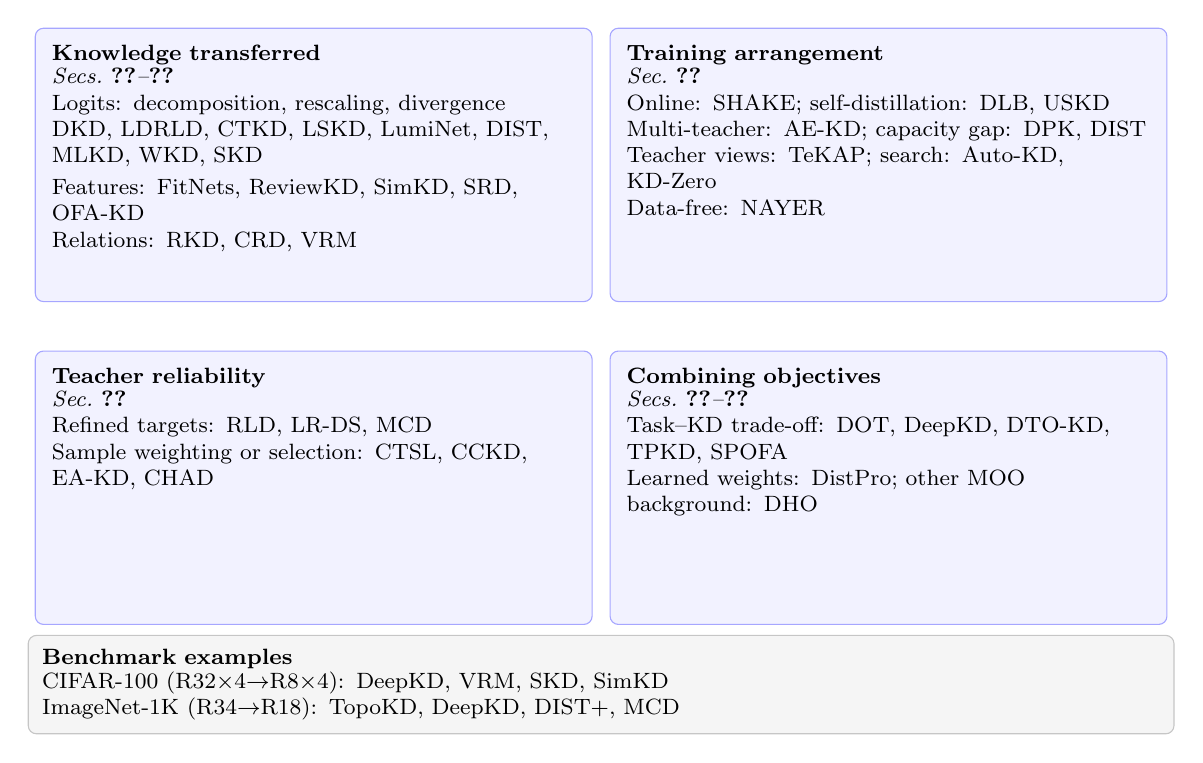
\begin{tikzpicture}[x=1cm,y=1cm,font=\footnotesize,
  card/.style={draw,rounded corners=3pt,fill=blue!5,draw=blue!35,
    text width=6.65cm,minimum height=3.45cm,inner sep=6pt,align=left},
  bench/.style={draw,rounded corners=3pt,fill=gray!8,draw=gray!45,
    text width=14.2cm,minimum height=1.05cm,inner sep=5pt,align=left}]
  \node[card] (knowledge) at (-3.65,2.05) {\parbox[t][3.05cm][t]{6.65cm}{\raggedright \textbf{Knowledge transferred}\\[-1pt]
    \textit{Secs.~\ref{sec:logit}--\ref{sec:feature}}\\
    Logits: decomposition, rescaling, divergence\\
    DKD, LDRLD, CTKD, LSKD, LumiNet, DIST, MLKD, WKD, SKD\\[2pt]
    Features: FitNets, ReviewKD, SimKD, SRD, \mbox{OFA-KD}\\
    Relations: RKD, CRD, VRM}};
  \node[card] (arrangement) at (3.65,2.05) {\parbox[t][3.05cm][t]{6.65cm}{\raggedright \textbf{Training arrangement}\\[-1pt]
    \textit{Sec.~\ref{sec:schemes}}\\
    Online: SHAKE; self-distillation: DLB, USKD\\
    Multi-teacher: AE-KD; capacity gap: DPK, DIST\\
    Teacher views: TeKAP; search: Auto-KD, \mbox{KD-Zero}\\
    Data-free: NAYER}};
  \node[card] (reliability) at (-3.65,-2.05) {\parbox[t][3.05cm][t]{6.65cm}{\raggedright \textbf{Teacher reliability}\\[-1pt]
    \textit{Sec.~\ref{sec:reliability}}\\
    Refined targets: RLD, LR-DS, MCD\\
    Sample weighting or selection: CTSL, CCKD, EA-KD, CHAD}};
  \node[card] (objectives) at (3.65,-2.05) {\parbox[t][3.05cm][t]{6.65cm}{\raggedright \textbf{Combining objectives}\\[-1pt]
    \textit{Secs.~\ref{sec:moo}--\ref{sec:kd_moo}}\\
    Task--KD trade-off: DOT, DeepKD, DTO-KD, TPKD, SPOFA\\
    Learned weights: DistPro; other MOO background: DHO}};
  \node[bench] (benchmarks) at (0,-4.55) {\textbf{Benchmark examples}\\[-1pt]
    CIFAR-100 (R32$\times$4$\to$R8$\times$4): DeepKD, VRM, SKD, SimKD\\
    ImageNet-1K (R34$\to$R18): TopoKD, DeepKD, DIST+, MCD};
\end{tikzpicture}

\caption{Overlapping dimensions used to organise the survey: knowledge transferred, training arrangement, teacher reliability and objective combination. The benchmark strip gives representative CIFAR-100 and ImageNet-1K methods discussed in Sec.~\ref{sec:benchmarks}. Examples include historical background and included 2022--2026 methods; publication status is discussed in the text and registry. Table~S2 lists all 112 records.}
\label{fig:taxonomy}
\end{figure}
% --- end Table I / Fig. 1 (T4) ---
